%! Author = itgramic
%! Date = 03.01.24

% Preamble
\chapter{Generell}
\begin{flushleft}
    Grundsätzlich verlauft der Patch auf den Test- und Produktivservern gleich ab.
    Die Services auf dem zweiten Server dürfen erst gestoppt werden, wenn der \Gls{JBoss}-Service auf dem ersten Server vollständig einsatzbereit ist und
    verbindungen annimmt.
\end{flushleft}
\begin{flushleft}
    Es gibt leider keine Garantie dafür, das die \Gls{JBoss}-Services laufen, wenn der Windows-Service läuft.
    Um zu Prüfen, ob der \Gls{JBoss}-Service an sich lauffähig ist, gibt es mehrere Indikatoren.
\end{flushleft}
\begin{flushleft}
    Zum einen gibt es im standalone-Verzeichnis das Subverzeichnis deployments in welchem gewisse Files auskunft über die Gesundheit des Nodes geben.
    Diese sind wie folgt zu finden:
    \dirtree{%
        .1 /.
        .2 laufwerk.
        .3 phoenix-server-<system>-<version>.
        .4 <node>.
        .5 standalone.
        .6 deployments.
    }
\end{flushleft}
\begin{flushleft}
    Bei einem geglückten Deployment eines Nodes muss ein \textit{phoenix.ear}- und \textit{phoenix.ear.deployed}-File vorhanden sein.\\Bei einem Fehler wiederum wird i.d.R. \textit{phoenix.ear.failed}-File erzeugt.
    \begin{figure}[H]
        \centering
        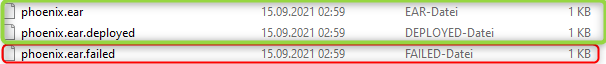
\includegraphics[width=1\linewidth]{source/general/deployments}
        \caption{Deployment-Status}
        \label{fig:deployment-status}
    \end{figure}
    Das entsprechende Mail ist im Anhang in folgendem Kapitel zu finden: \autoref{chap:811534244}
\end{flushleft}
\begin{flushleft}
    Allerdings ist dies nicht immer 100\% verlässlich.
    Die sicherste Methode, um die Funktionsfähigkeit eines Nodes resp.
    Servers zu testen besteht darin, die \textit{Workstation.exe} nur noch auf den entsprechenden Node resp.
    Server verbinden zu lassen.
    Die Verbindung wird ins \textit{Workstation.ini} geschrieben, welches wie üblich hier zu finden ist:
\end{flushleft}
\begin{flushleft}
    \dirtree{%
        .1 /.
        .2 C:\textbackslash.
        .3 Program Files (x86).
        .4 <Phoenix7-Verzeichnis>.
        .5 Workstation.ini.
    }
\end{flushleft}
\begin{flushleft}
    Im Ini stehen die \Gls{JBoss}-Server und Nodes im Eintrag \textit{-Dphoenix.server.nodes}.
    Hier das Beispiel des Produktiven Ini-Files:
    \lstset{style=gra_codestyle}
    \begin{lstlisting}[language=sh, caption=Workstation.ini PROD Beispiel,captionpos=b,label={lst:workstation.ini-prod-beispiel},breaklines=true]
    -clean
    -data
    @noDefault
    -configuration c:/temp/phoenix/prod_7_23_1/eclipse/configuration
    -nl
    de_CH
    -vmargs
    -Dorg.eclipse.update.reconcile=false
    -Dphoenix.db=Phoenix
    -Dphoenix.application.workspace.createdir=true
    -Dphoenix.application.workspace=\\\\phoenix\workspace\prod_7_23_1
    -Dphoenix.login.usernamefile=%APPDATA%/Phoenix/login_username_prod
    -Dphoenix.server.nodes=sks0020:8443,sks0021:8443,sks0020:8543,sks0021:8543
    -Djavax.net.ssl.trustStore=C:\Program Files (x86)\Phoenix7\truststore.jks
    -Dphoenix.login.enableLDAP=true
    -Dphoenix.application.winlogin=true
    -XX:-CreateMinidumpOnCrash
    \end{lstlisting}
\end{flushleft}
\begin{flushleft}
    Am Einfachsten ist, man erstellt sich drei Ini-Files, eines für beide Server zusammen im Cluster und eines pro Server.
    Dann braucht man nur die Files umzubennen und kann rasch Testen.
\end{flushleft}
\begin{flushleft}
    \begin{mdframed}
    Vorsichht!\\Es kann vorkommen, dass jeder Server für sich alleine Lauffähig ist aber im Cluster-Verbund keine Anmeldung möglich ist!\\
    Daher sollte nach einem Reboot nebst der Lauffähigkeit der einzelnen Nodes auch immer der Cluster getestet werden!
    \end{mdframed}
\end{flushleft}
\begin{flushleft}
    Obwohl die Server mittels \Gls{Ivanti} betankt werden, kann es vorkommen, dass nicht alle Patches geladen wurden.
    Um sicherzustellen, dass das System komplett sauber gepatched wurde, sollte man immer noch auf Updates Prüfen.

    Geprüft wird Normal via Suche:
    \begin{figure}[H]
        \centering
        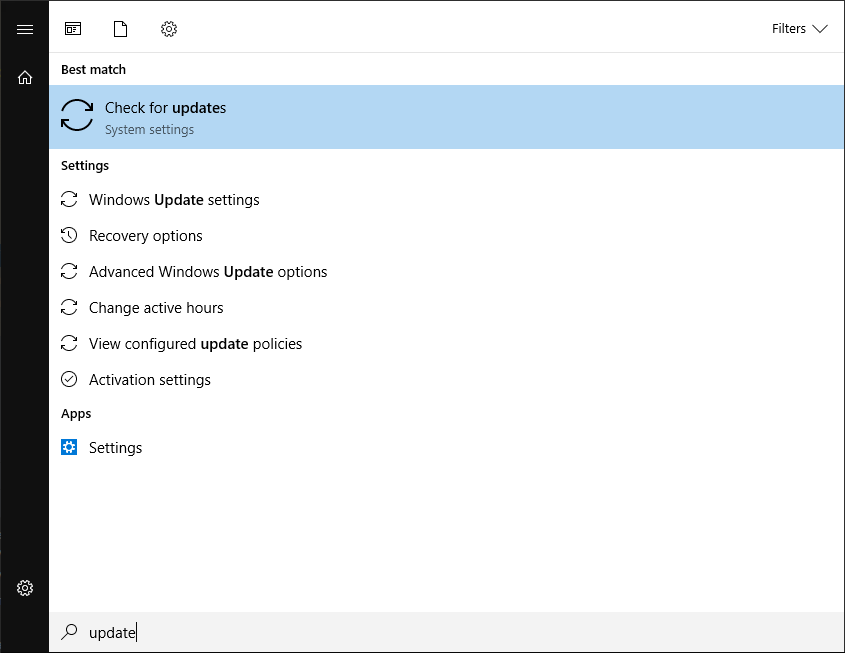
\includegraphics[width=1\linewidth]{source/general/search_for_updates}
        \caption{Check-Updates}
        \label{fig:check-updates}
    \end{figure}

    Solange noch Updates wie folgt vorhanden sind, müssen diese manuell nachgeladen und installiert werden:
    \begin{figure}[H]
        \centering
        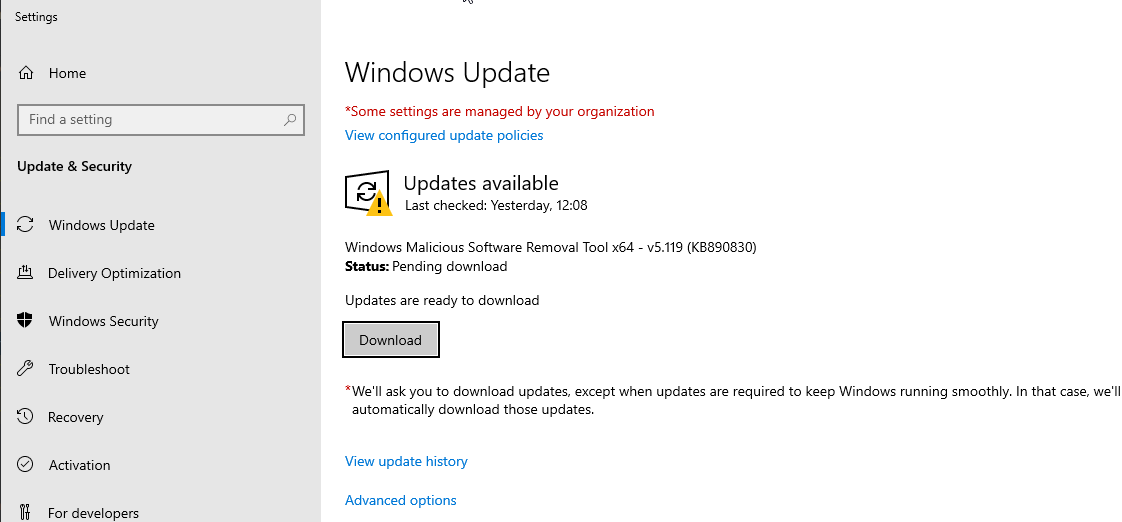
\includegraphics[width=1\linewidth]{source/general/updates_available}
        \caption{Updates available}
        \label{fig:updates-available}
    \end{figure}

    Dies ist aber äusserst selten der Fall.

    \begin{mdframed}
    Vorsichht!\\Sollte es trotzdem mal vorkommen, niemals die \Gls{RDP}-Verbindung schliessen!\\Ansonsten wird es unmöglich sein, den Server gezielt zu rebooten.
    \end{mdframed}

\end{flushleft}